% The flow past a circular cylinder generates a vortex street that is known as the Von K´arm´an
% Vortex Street. In this lab, we will simulate the steady state solution of this vortex shedding phenomenon based on a laminar flow of air at 25◦C over a 2D circular cylinder. The
% schematics of the problem is shown in Figure 1, where the cylinder diameter (D) is 10 mm,
% the free stream velocity is U∞ = 0.24 m/s

% PART I. Problem Setup
% The first step in setting up a computational simulation is to understand the problem and
% calculate important parameters. Then, the problem is replicated by designing a correct CAD
% model that is used for mesh generation. This is followed by assigning boundary conditions
% and initial conditions to solve the Navier-Stokes equation.
% Considering the setup in Figure 1, complete the following tasks:
% Task 1.1. Calculate the problem Reynolds number (Re = U∞D/ν) and confirm that the
% flow is laminar.
% Task 1.2. Open ANSYS Workbench and define a new project based on ANSYS Fluent.
% Task 1.3. Generate a CAD model for dimensions and the simulation setup discussed above
% (i.e., Figure 1) using ANSYS Design Modeler.
% Task 1.4. Generate a moderately fine mesh for the geometry built in the previous step.
% The minimum element length is D/5, which should be labeled “Grid 1”. You should place
% 5 Prism Layers (Inflation Layers) around the cylinder at a “Transition Ratio” of 0.25, and
% “Growth Rate” of 1.2.
% Task 1.5. In ANSYS Fluent, assign the relevant boundary conditions to the domain as it
% has been described in Figure 1. The outlet boundary condition is “Outlet” with a relative
% “Gauge Pressure” of 0 atm.
% Task 1.6. The convergence threshold residual should be set at 10−4
% . The lower this value,
% more accurate the simulations are and more computational resources to complete the simulations.
% Task 1.7. Under “Monitors”, set a “Report Plot” for plotting drag force applying on the
% cylinder against number of iterations. Note that the drag force needs to be defined in “Report
% Definitions” before being set.
% Task 1.8. Assign the standard initialization of ux = 0, uy = 0, and pg = 0 (gauge pressure)
% to the entire domain.
% % Task 1.9. The maximum number of iterations recommended is 1000.
% Based on the setup from PART I, complete the following task:
% Task 2.1. Complete the simulation of laminar flow of air over a 2D circular cylinder using
% “Grid 1”. The pressure-velocity coupling scheme should be set as “Coupled”. Spatial discretization methods for pressure and momentum should be second order accurate. You can
% change the solver method under Solution in ANSYS Fluent.
% Task 2.2. Once the simulation is complete, proceed to ANSYS CFD-Post for post-processing
% of the data. Obtain or calculate the following:
% (I) Calculate the Mean Drag Force (force acting in the x−direction) acting on the cylinder.
% (II) Calculate the Mean Drag Coefficient (Cd = FD/(0.5ρU2
% ∞D)) for the cylinder.
% (III) Draw the plot of mean streamwise (x−direction) velocity (u) along the wake centerline
% (the horizontal line that starts at the center of the cylinder and extends to the end of the
% computational domain - only in the x−direction). Note the x−location at which this
% line crosses zero for the first time. This is referred to as the “Mean Recirculation Length”
% (Lr). Normalize this number using the problem characteristic length, which is the
% cylinder diameter (D).
% (IV) Create a contour plot of mean pressure (p) in the wake. Adjust the values of maximum
% and minimum pressure so that the recirculation vortex is distinguishable from the flow.
% (V) Has the solution converged? Do you believe that the results illustrate a steady state
% solution of the wake? Please justify your answer.
% NOTE: The extent of the recirculation (mean) vortex in the x−direction, which was identified by the contour plot of pressure, should be identical to the value of Lr.
% PART III. Grid Independence Analysis
% Task 3.1. Create a new case in ANSYS Workbench called “Grid 2” and changed the
% minimum mesh size to D/10 ≈ 1 mm. You should place at least 10 Prism Grid around the
% cylinder. Then, redo all tasks and complete the simulations. Re-generate all the plots and
% calculations from Task 2.2 for “Grid 2”.
% Task 3.2. Create two more case in ANSYS Workbench “Grid 3” and “Grid 4” using ANSYS
% Fluent and change the minimum mesh size to D/15 ≈ 0.667 mm and D/20 ≈ 0.5 mm.
% Complete the simulations and re-generate all the plots and calculations from Task 2.2 for
% “Grid 3” and “Grid 4”.
% Task 3.3. Create a table that includes the number of elements (n), coefficient of drag (Cd),
% the mean recirculation length (Lr), and their percentage of change with respect to “Grid 1”.
% 3
% Comment on how they differ for the four grids. Which grid should be used for simulating
% this laminar flow? Why? Please justify your answer.
% NOTE: This process is commonly referred to as the “Grid Independence Analysis”. The
% final selected grid will be used for the main simulation and to obtain results.

\section*{Part I. Problem Setup}
\subsection*{Task 1.1}
\textit{Calculate the problem Reynolds number (Re = $U_\infty D/\nu$) and confirm that the flow is laminar.}

The working fluid is air. The properties of air at 25°C and 1 atm are taken from a textbook \cite{Cengel2017-jf}.
\begin{align*}
    \rho &= 1.184 \text{ kg/m}^3 \\
    \mu &= 1.562 \times 10^{-5} \text{ kg/ms} \\
    \nu &= \frac{\mu}{\rho} = 1.318 \times 10^{-5} \text{ m}^2/\text{s}
\end{align*}

The Reynolds number is calculated as
\begin{align*}
    \text{Re} &= \frac{U_\infty D}{\nu} \\
    &= \frac{0.24  \times 0.1}{1.318 \times 10^{-5}} \\
    &= 1820.9
\end{align*}
This is less than the critical Reynolds number of 2000, so the flow is laminar.

\subsection*{Task 1.3}
\textit{Generate a CAD model for dimensions and the simulation setup discussed above (i.e., Figure 1) using ANSYS Design Modeler.}
\begin{figure}[H]
    \centering
    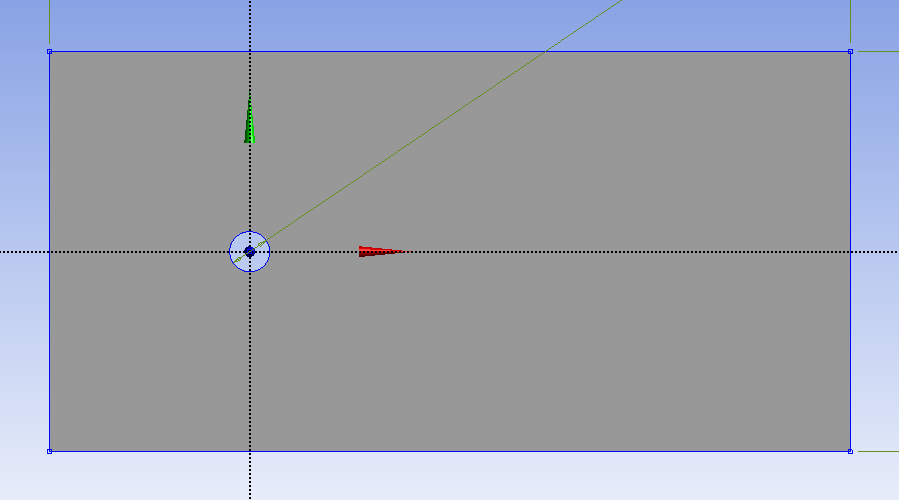
\includegraphics[width=0.8\textwidth]{Questions/Figures/geometry.png}
    \caption{Geometry for the Flow Past a Circular Cylinder}
\end{figure}

\subsection*{Task 1.4}
\textit{Generate a moderately fine mesh for the geometry built in the previous step. The minimum element length is $D/5$, which should be labeled “Grid 1”. You should place 5 Prism Layers (Inflation Layers) around the cylinder at a “Transition Ratio” of 0.25, and “Growth Rate” of 1.2.}
\begin{figure}[H]
    \centering
    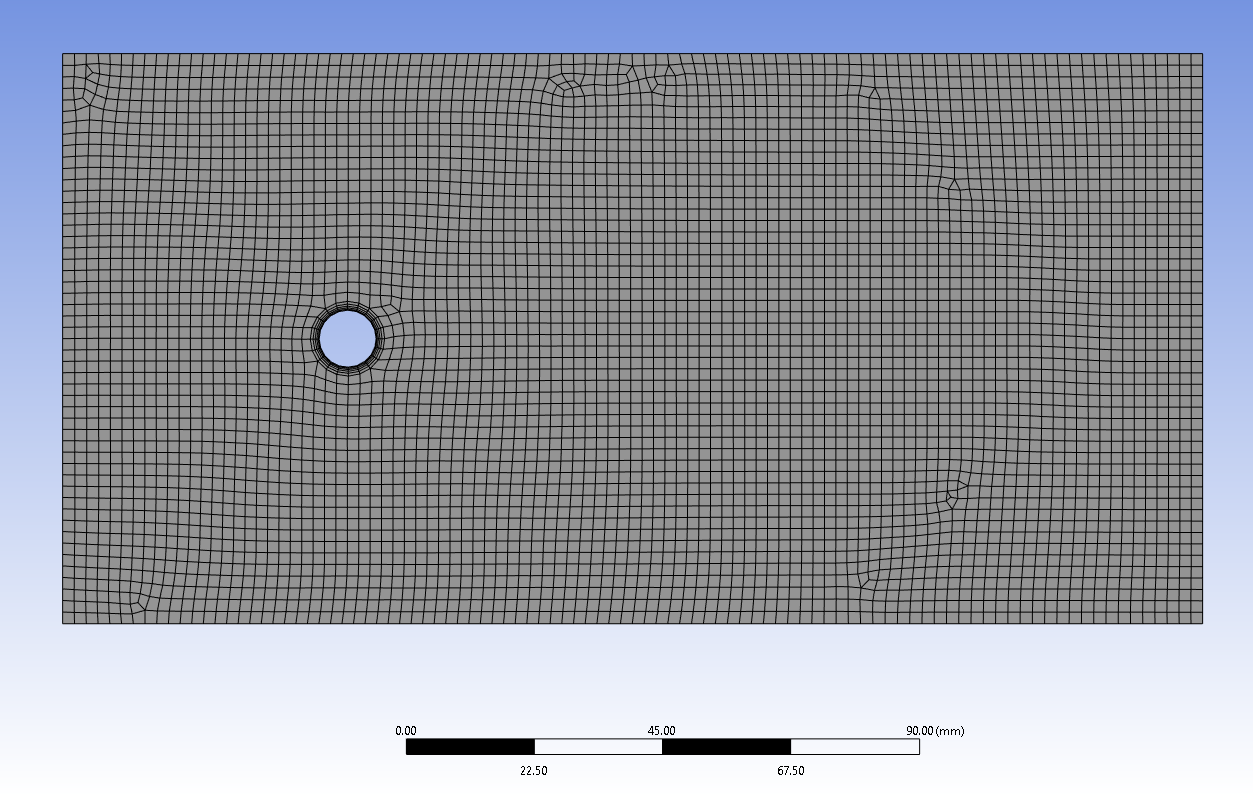
\includegraphics[width=0.8\textwidth]{Questions/Figures/mesh with grid 1.png}
    \caption{Mesh for Grid 1}
\end{figure}

\section*{Part II. Reference Simulation}

\subsection*{Summary for Grids 1, 2, 3, and 4}
\begin{table}[H]
    \centering
    \caption{Summary of Results for Grids 1, 2, 3, and 4 (for ease of marking)}
    \begin{tabular}{ccccc}
        \toprule
        Grid & $F_D$ & $C_d$ & $L_r$ \\ 
        & (N) & & \\
        \midrule
        1 & $4.08667 \times 10^{-7}$ & $1.2 \times 10^{-4}$ & 32.5 \\
        2 & $3.97047 \times 10^{-7}$ & $1.16 \times 10^{-4}$ & 43.0 \\
        3 & $3.97047 \times 10^{-7}$ & $1.16 \times 10^{-4}$ & 44.0 \\
        4 & $3.92433 \times 10^{-7}$ & $1.15 \times 10^{-4}$ & 44.0 \\
        \bottomrule
    \end{tabular}
\end{table}

\subsection*{Task 2.1}
\textit{Complete the simulation of laminar flow of air over a 2D circular cylinder using “Grid 1”. The pressure-velocity coupling scheme should be set as “Coupled”. Spatial discretization methods for pressure and momentum should be second order accurate. You can change the solver method under Solution in ANSYS Fluent.}
\begin{figure}[H]
    \centering
    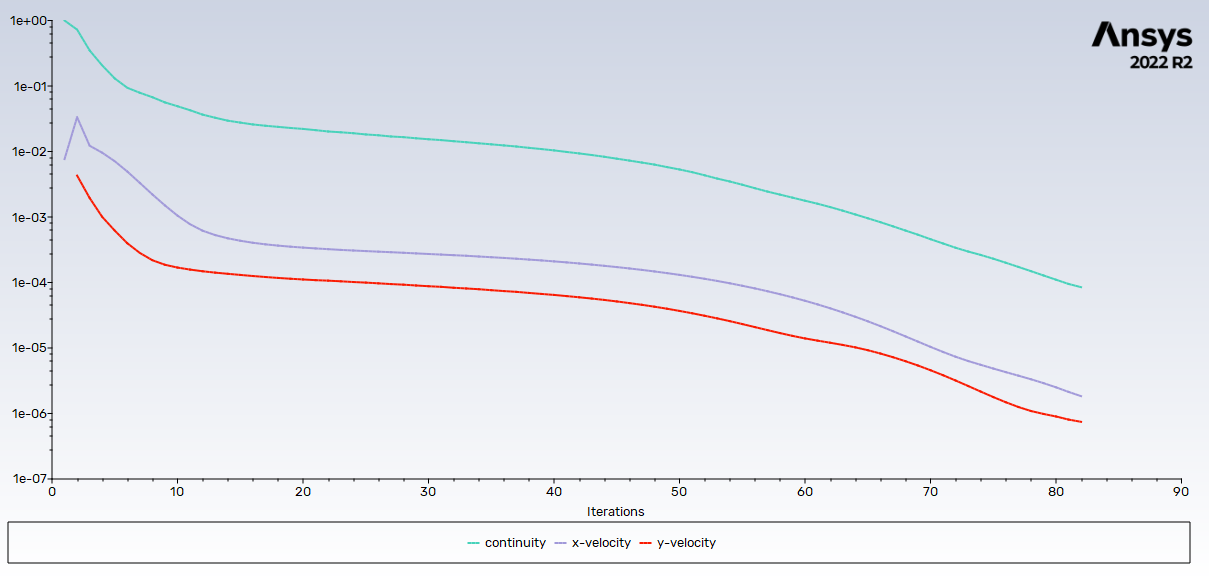
\includegraphics[width=0.8\textwidth]{Questions/Figures/residuals grid 1.png}
    \caption{Residuals for Grid 1}
\end{figure}

\subsection*{Task 2.2}
\textit{(I) Calculate the Mean Drag Force (force acting in the $x$-direction) acting on the cylinder.}
\begin{figure}[H]
    \centering
    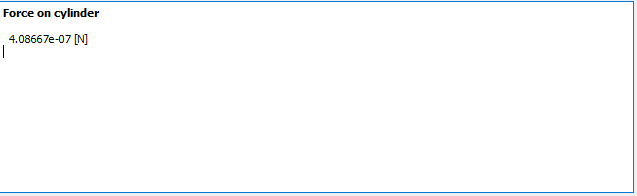
\includegraphics[width=0.8\textwidth]{Questions/Figures/force on cylinder grid 1.png}
    \caption{Mean Drag Force for Grid 1}
\end{figure}

\textit{(II) Calculate the Mean Drag Coefficient ($C_d = F_D/(0.5\rho U_\infty^2 D)$) for the cylinder.}

By direct calculation, the mean drag coefficient is
\begin{align*}
    C_{d1} &= \frac{F_{D1}}{0.5\rho U_\infty^2 D} \\
    &= \frac{4.08667 \times 10^{-7}}{0.5 \times 1.184 \times 0.24^2 \times 0.1} \\
    &= 1.2 \times 10^{-4}
\end{align*}

\textit{(III) Draw the plot of mean streamwise ($x$-direction) velocity ($u$) along the wake centerline (the horizontal line that starts at the center of the cylinder and extends to the end of the computational domain - only in the $x$-direction). Note the $x$-location at which this line crosses zero for the first time. This is referred to as the “Mean Recirculation Length” ($L_r$). Normalize this number using the problem characteristic length, which is the cylinder diameter ($D$).}
\begin{figure}[H]
    \centering
    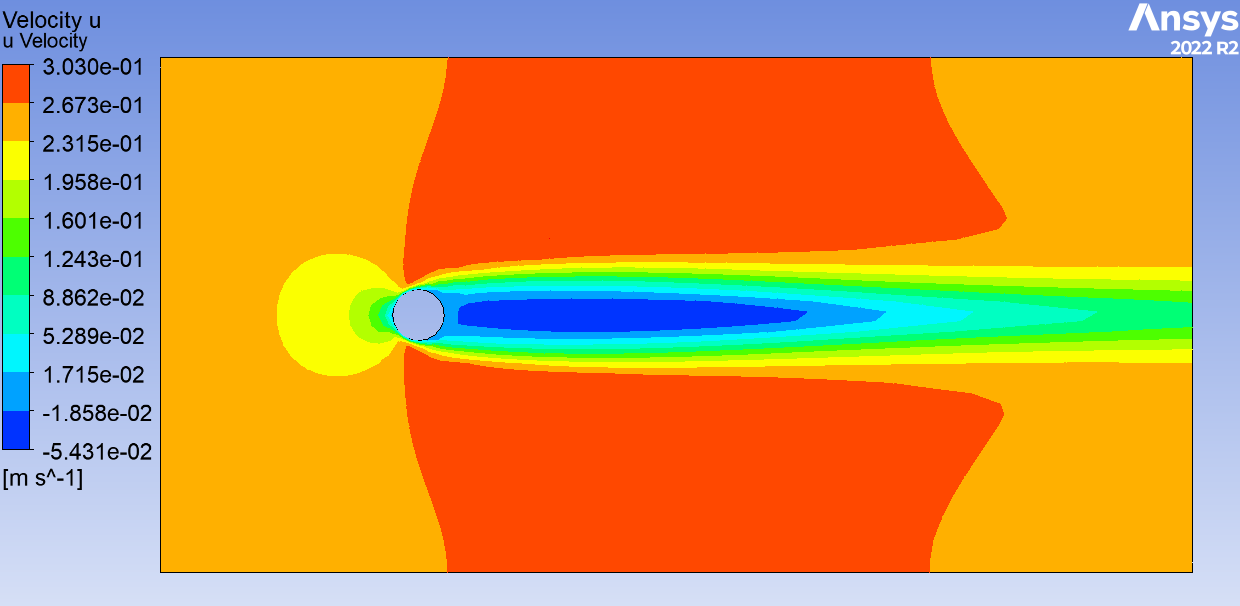
\includegraphics[width=0.8\textwidth]{Questions/Figures/u velocity contour grid 1.png}
    \caption{Mean Streamwise Velocity Contour for Grid 1}
\end{figure}
\begin{figure}[H]
    \centering
    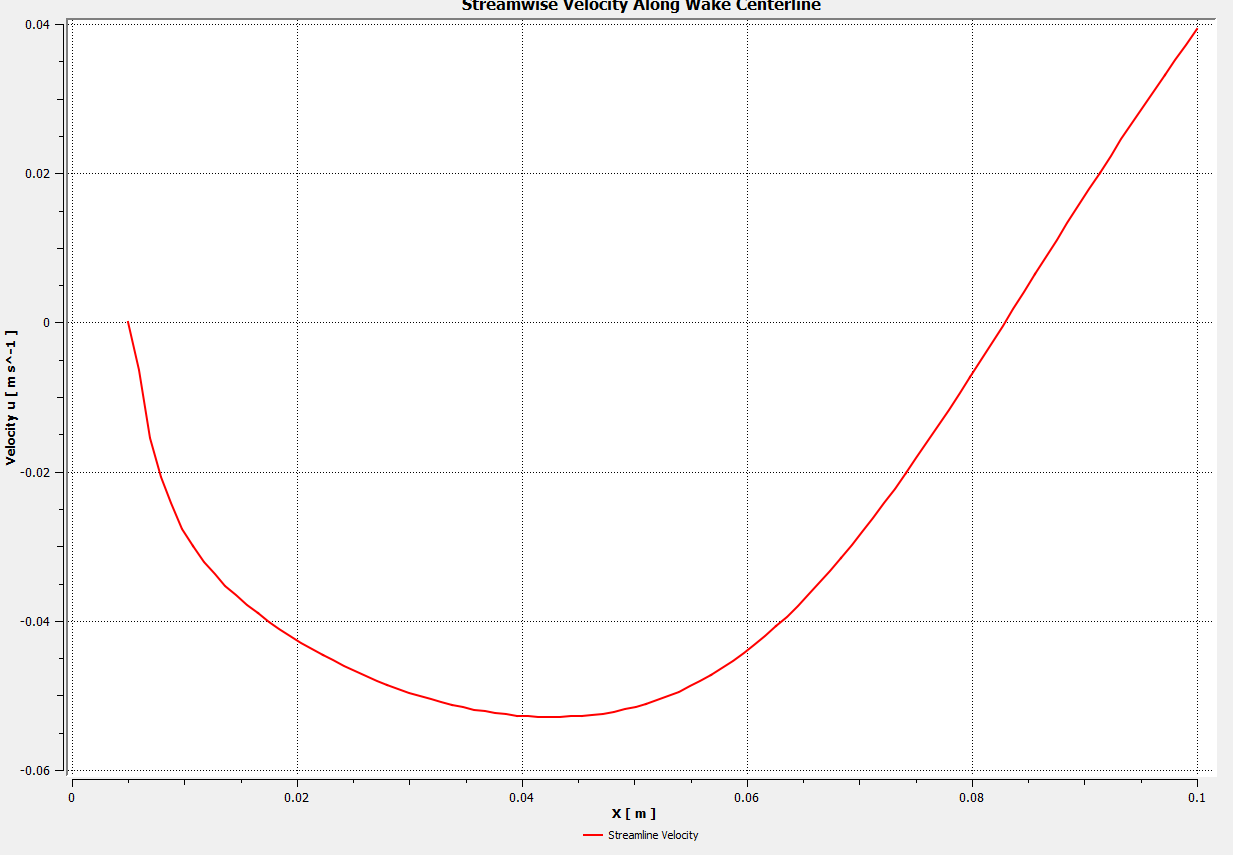
\includegraphics[width=0.8\textwidth]{Questions/Figures/plot with grid 1.png}
    \caption{Mean Streamwise Velocity for Grid 1}
\end{figure}
From the plot, the recirculation length is approximately
\begin{align*}
    L_{r1} &= \frac{0.0825 - 0.05}{0.001} \\
    &=\boxed{32.5}
\end{align*}

\textit{(IV) Create a contour plot of mean pressure ($p$) in the wake. Adjust the values of maximum and minimum pressure so that the recirculation vortex is distinguishable from the flow.}
\begin{figure}[H]
    \centering
    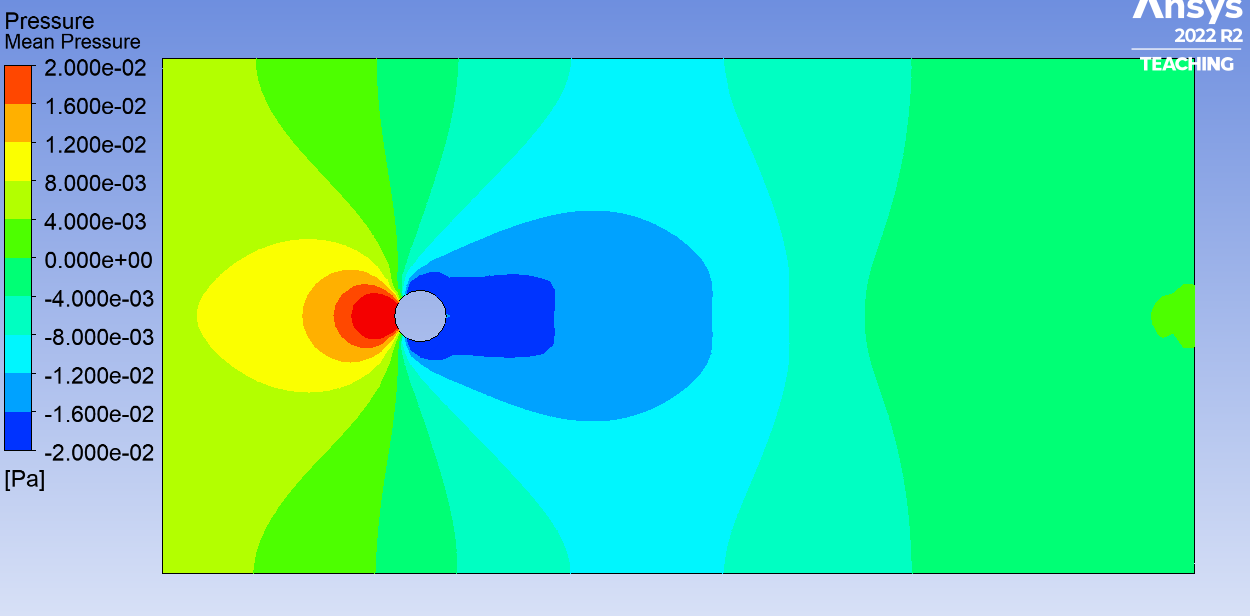
\includegraphics[width=0.8\textwidth]{Questions/Figures/mean pressure grid 1.png}
    \caption{Mean Pressure Contour for Grid 1}
\end{figure}

\textit{(V) Has the solution converged? Do you believe that the results illustrate a steady state solution of the wake? Please justify your answer.}
\begin{figure}[H]
    \centering
    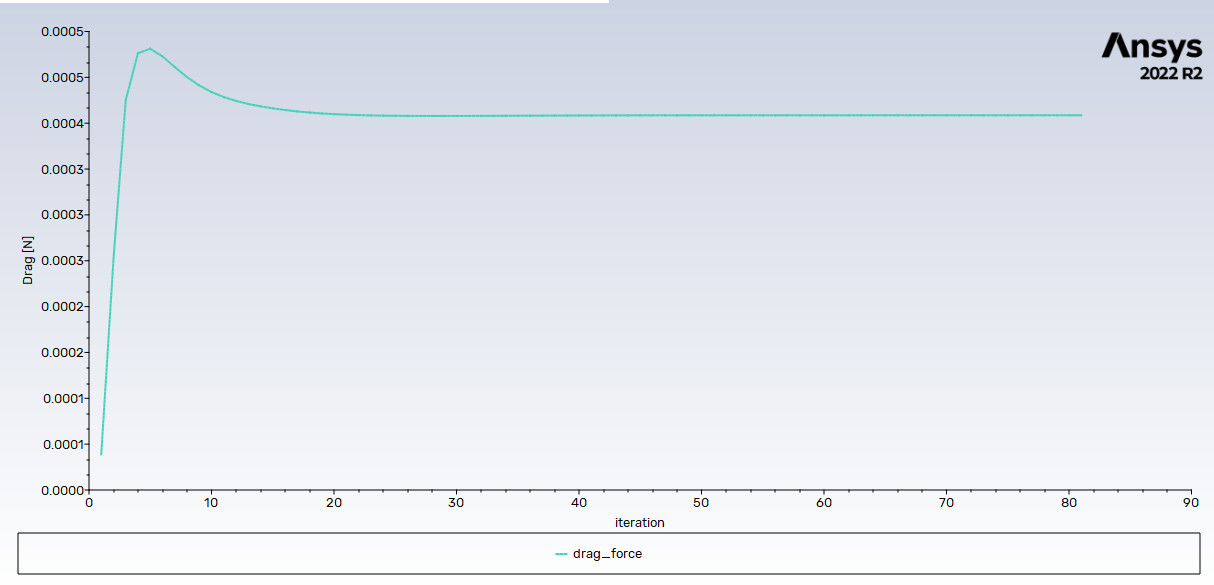
\includegraphics[width=0.8\textwidth]{Questions/Figures/drag force grid 1.png}
    \caption{Drag force over iterations for Grid 1}
\end{figure}
The drag force converges to a constant steady-state value. 

\section*{Part III. Grid Independence Analysis}
\subsection*{Task 3.1}
\textit{Create a new case in ANSYS Workbench called “Grid 2” and changed the minimum mesh size to $D/10 \approx 1$ mm. You should place at least 10 Prism Grid around the cylinder. Then, redo all tasks and complete the simulations. Re-generate all the plots and calculations from Task 2.2 for “Grid 2”.}
\begin{figure}[H]
    \centering
    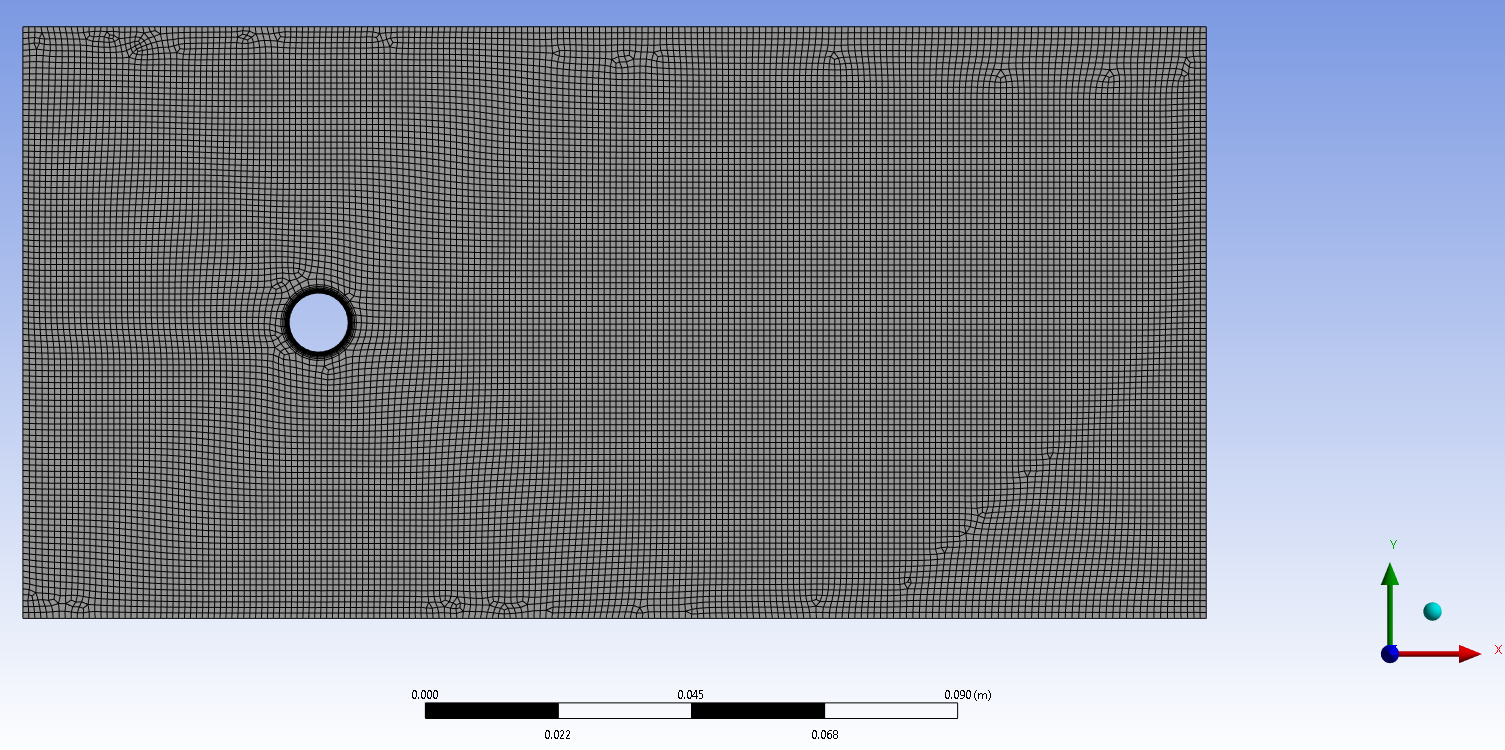
\includegraphics[width=0.8\textwidth]{Questions/Figures/mesh with grid 2.png}
    \caption{Mesh for Grid 2}
\end{figure}
\begin{figure}[H]
    \centering
    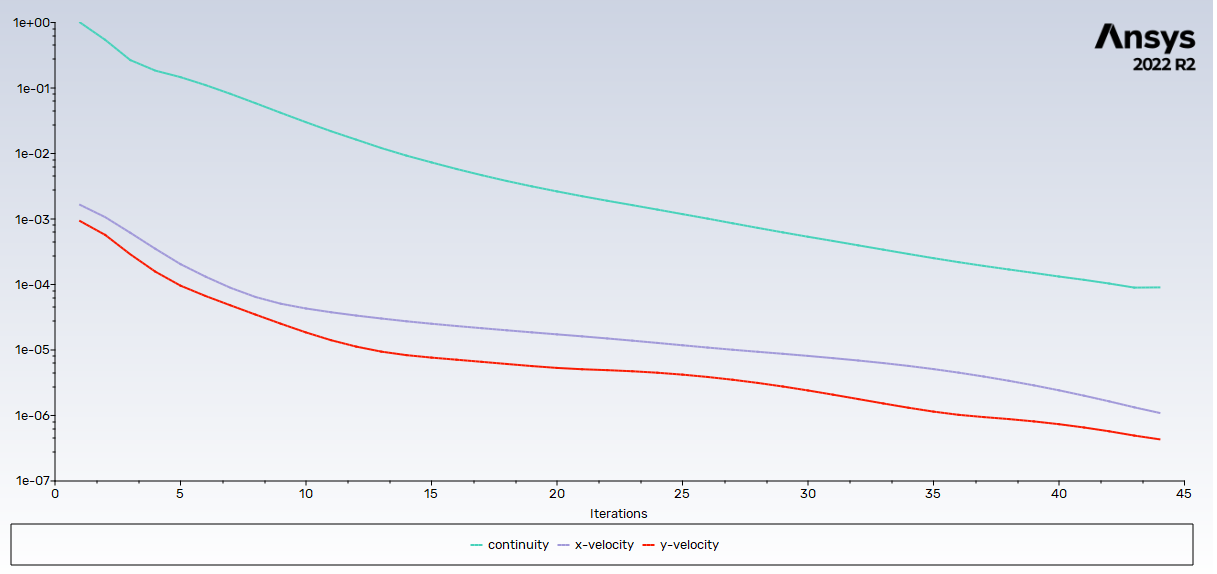
\includegraphics[width=0.8\textwidth]{Questions/Figures/residuals grid 2.png}
    \caption{Residuals for Grid 2}
\end{figure}
\begin{figure}[H]
    \centering
    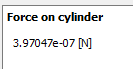
\includegraphics[width=0.8\textwidth]{Questions/Figures/force on cylinder grid 2.png}
    \caption{Mean Drag Force for Grid 2}
\end{figure}
By direct calculation, the mean drag coefficient is
\begin{align*}
    C_{d2} &= \frac{F_{D2}}{0.5\rho U_\infty^2 D} \\
    &= \frac{3.97047 \times 10^{-7}}{0.5 \times 1.184 \times 0.24^2 \times 0.1} \\
    &= 1.16 \times 10^{-4}
\end{align*}
From the plot, the recirculation length is approximately
\begin{align*}
    L_{r2} &= \frac{0.093 - 0.05}{0.001} \\
    &=\boxed{43.0}
\end{align*}
\begin{figure}[H]
    \centering
    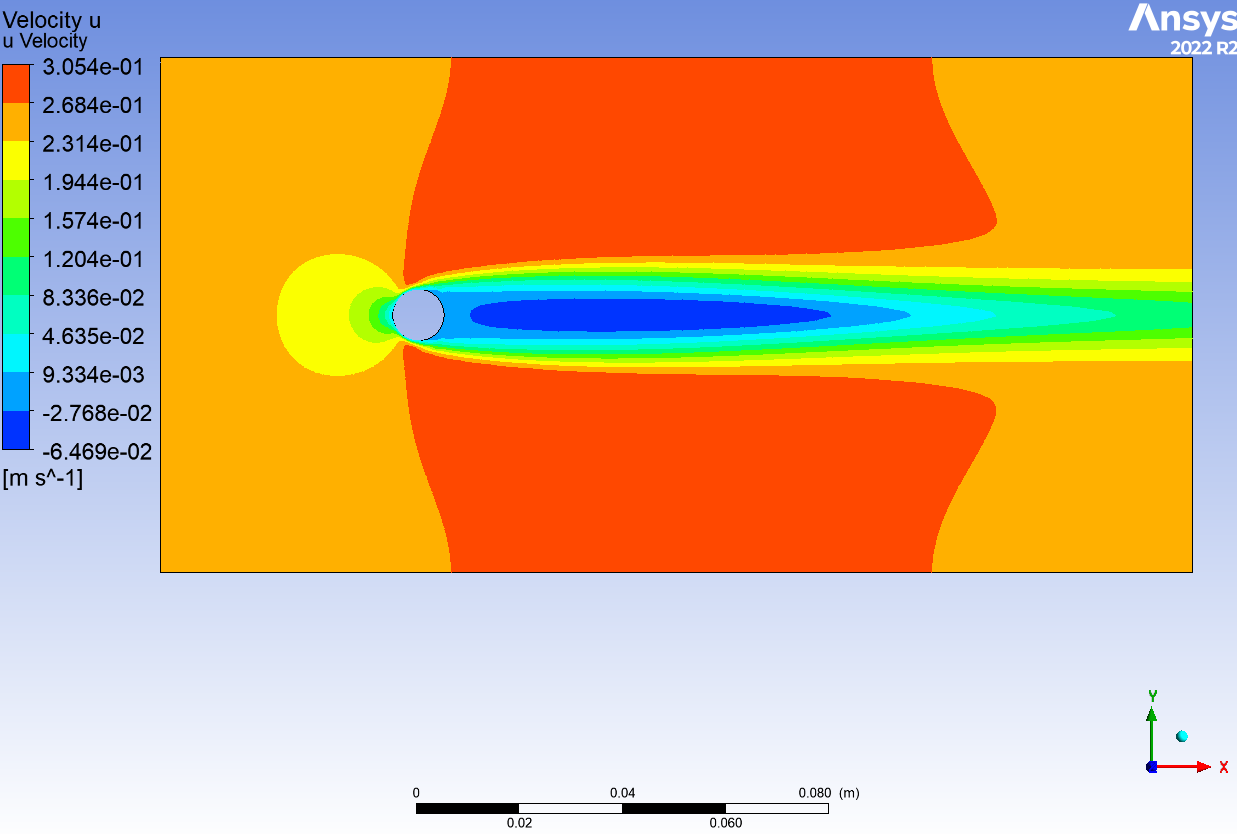
\includegraphics[width=0.8\textwidth]{Questions/Figures/u velocity contour grid 2.png}
    \caption{Mean Streamwise Velocity Contour for Grid 2}
\end{figure}
\begin{figure}[H]
    \centering
    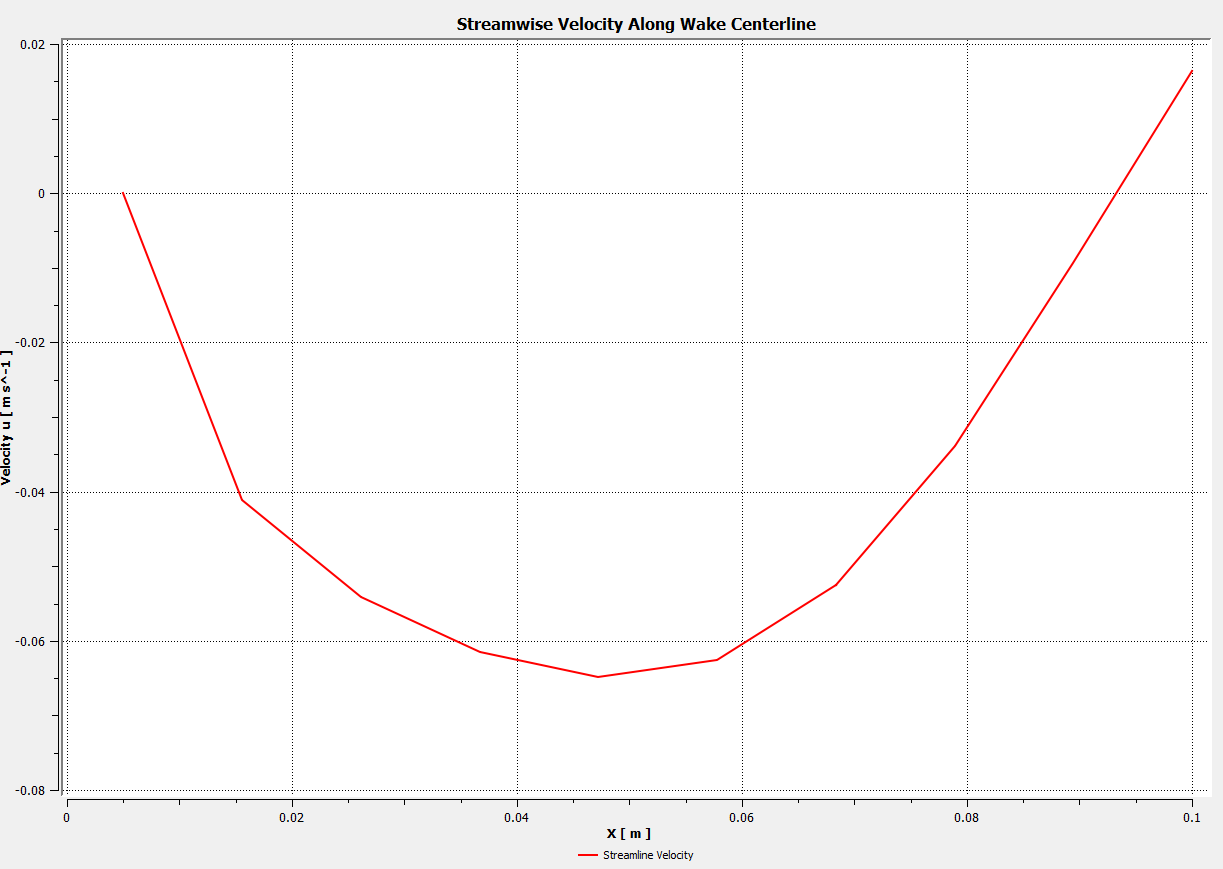
\includegraphics[width=0.8\textwidth]{Questions/Figures/plot with grid 2.png}
    \caption{Mean Streamwise Velocity for Grid 2}
\end{figure}
\begin{figure}[H]
    \centering
    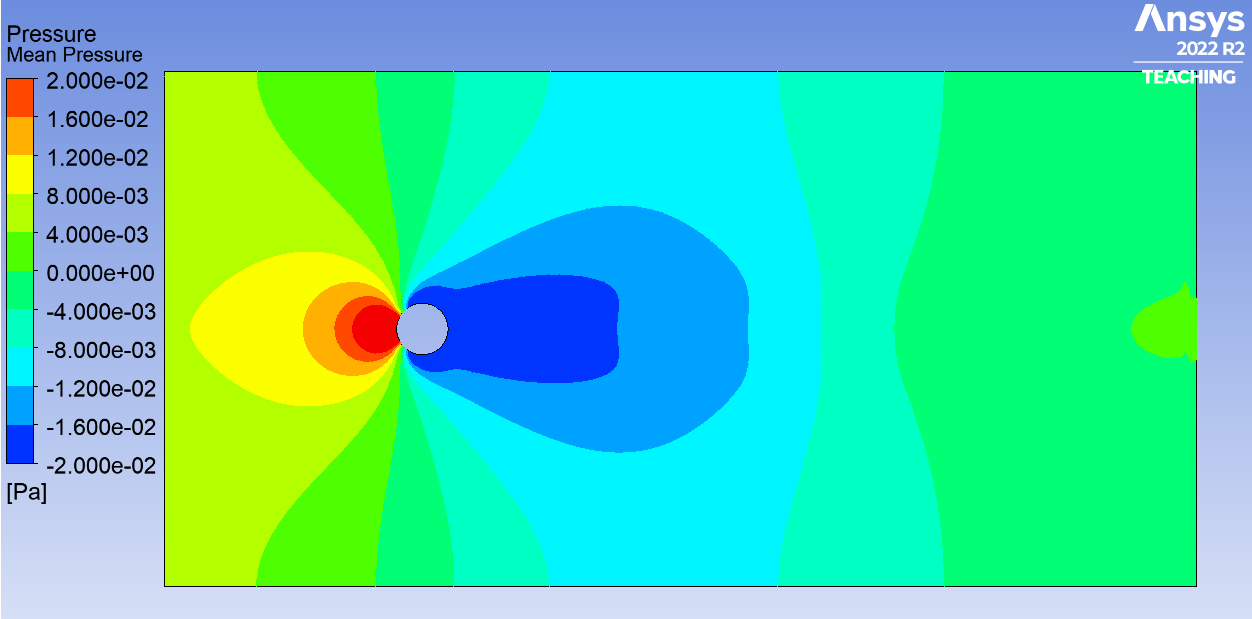
\includegraphics[width=0.8\textwidth]{Questions/Figures/mean pressure grid 2.png}
    \caption{Mean Pressure Contour for Grid 2}
\end{figure}

\subsection*{Task 3.2}
\textit{Create two more case in ANSYS Workbench “Grid 3” and “Grid 4” using ANSYS Fluent and change the minimum mesh size to $D/15 \approx 0.667$ mm and $D/20 \approx 0.5$ mm. Complete the simulations and re-generate all the plots and calculations from Task 2.2 for “Grid 3” and “Grid 4”.}

\subsubsection*{Grid 3}
\begin{figure}[H]
    \centering
    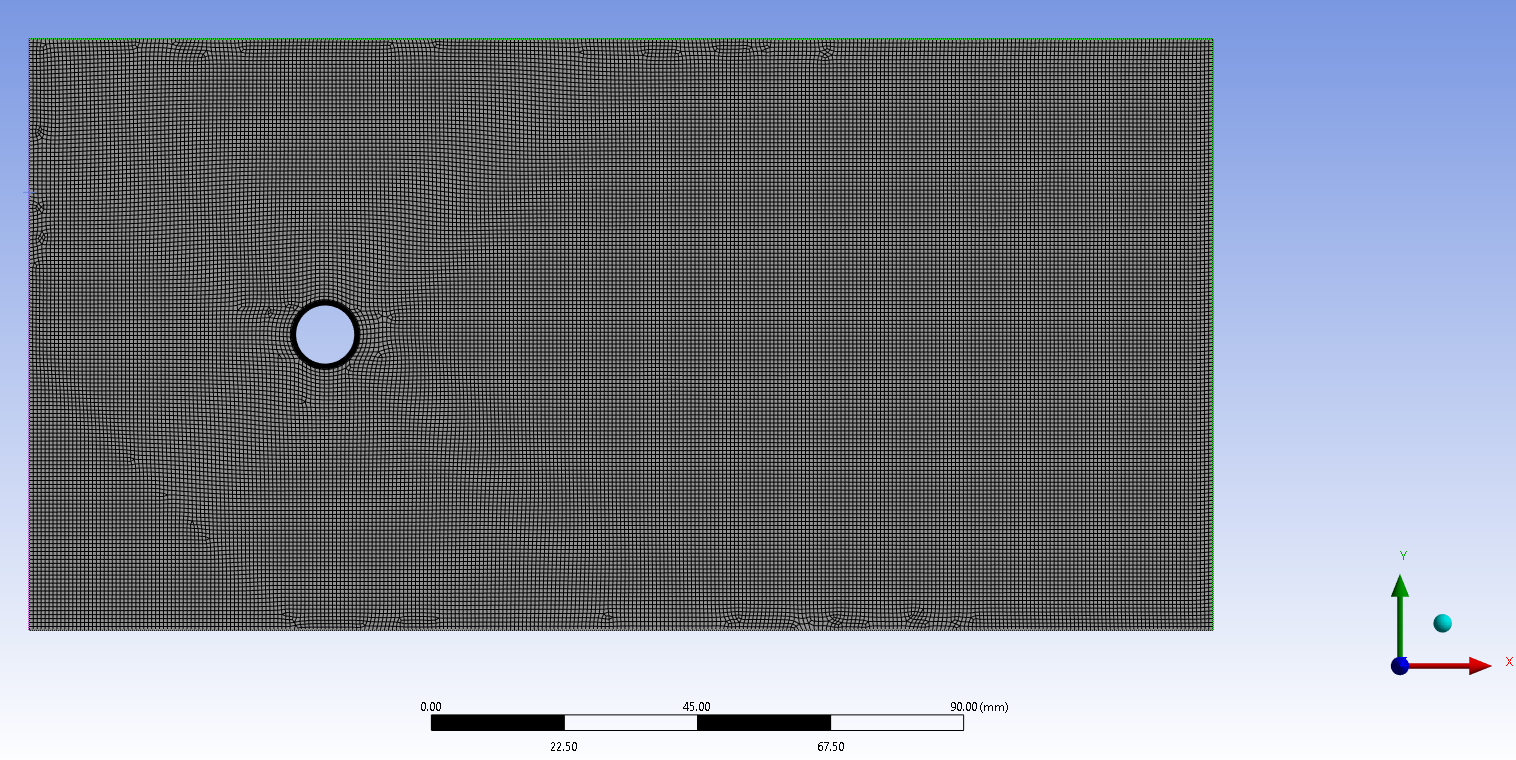
\includegraphics[width=0.8\textwidth]{Questions/Figures/mesh with grid 3.png}
    \caption{Mesh for Grid 3}
\end{figure}
\begin{figure}[H]
    \centering
    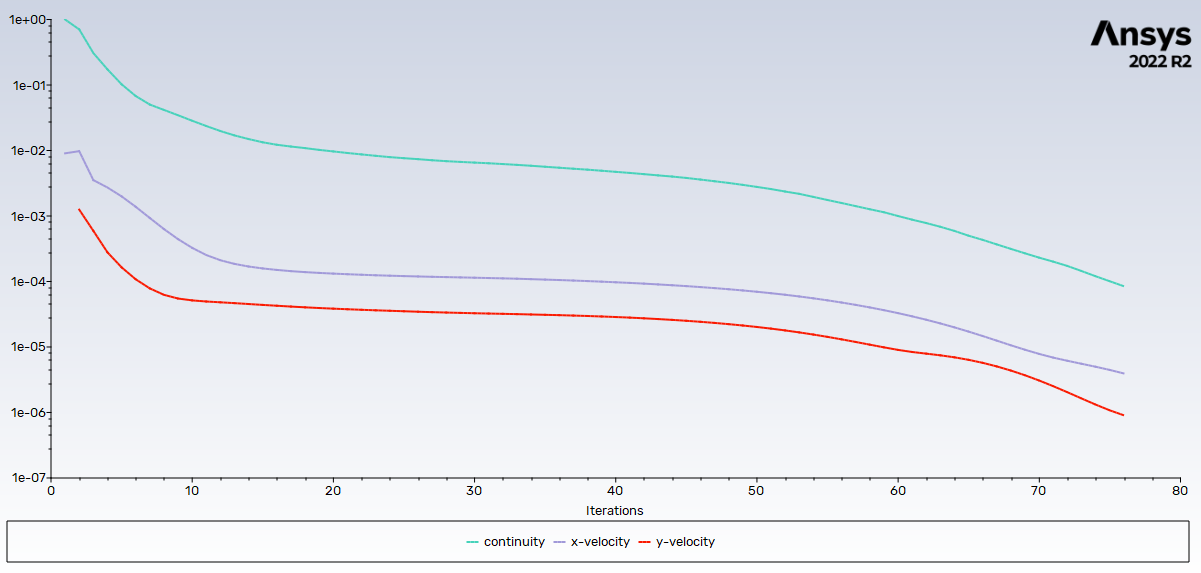
\includegraphics[width=0.8\textwidth]{Questions/Figures/residuals grid 3.png}
    \caption{Residuals for Grid 3}
\end{figure}
\begin{figure}[H]
    \centering
    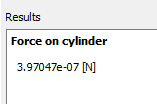
\includegraphics[width=0.8\textwidth]{Questions/Figures/force on cylinder grid 3.png}
    \caption{Mean Drag Force for Grid 3}
\end{figure}
By direct calculation, the mean drag coefficient is
\begin{align*}
    C_{d3} &= \frac{F_{D3}}{0.5\rho U_\infty^2 D} \\
    &= \frac{3.97047 \times 10^{-7}}{0.5 \times 1.184 \times 0.24^2 \times 0.1} \\
    &= 1.16 \times 10^{-4}
\end{align*}
From the plot, the recirculation length is approximately
\begin{align*}
    L_{r3} &= \frac{0.094 - 0.05}{0.001} \\
    &=\boxed{44.0}
\end{align*}
\begin{figure}[H]
    \centering
    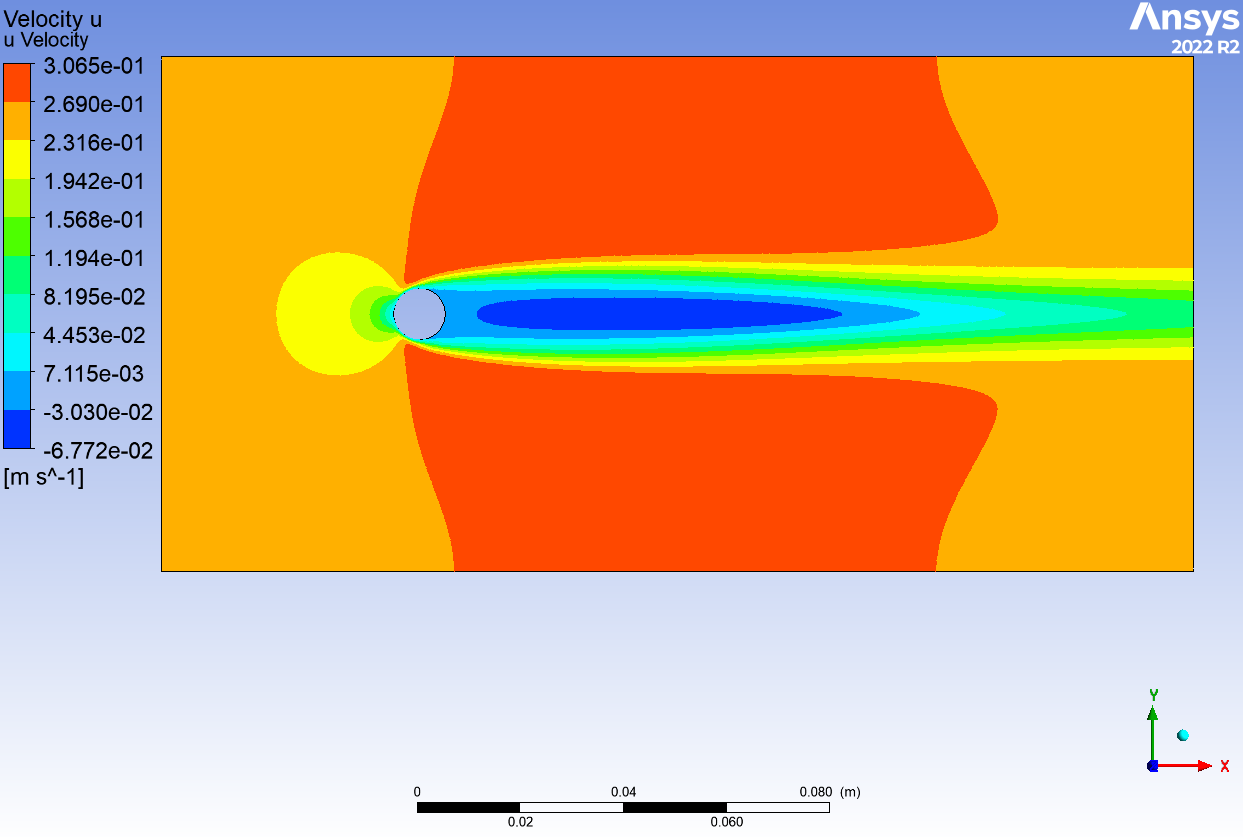
\includegraphics[width=0.8\textwidth]{Questions/Figures/u velocity contour grid 3.png}
    \caption{Mean Streamwise Velocity Contour for Grid 3}
\end{figure}
\begin{figure}[H]
    \centering
    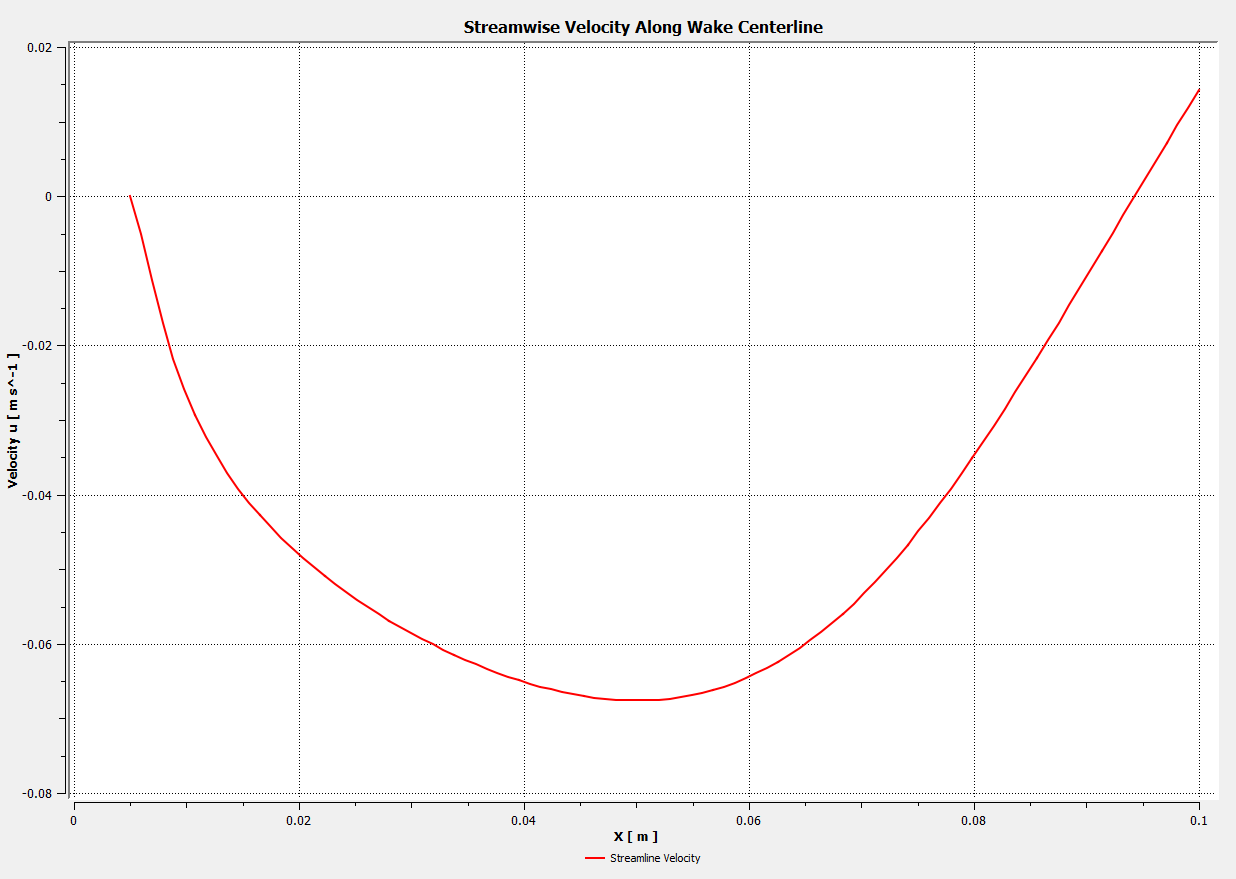
\includegraphics[width=0.8\textwidth]{Questions/Figures/plot with grid 3.png}
    \caption{Mean Streamwise Velocity for Grid 3}
\end{figure}
\begin{figure}[H]
    \centering
    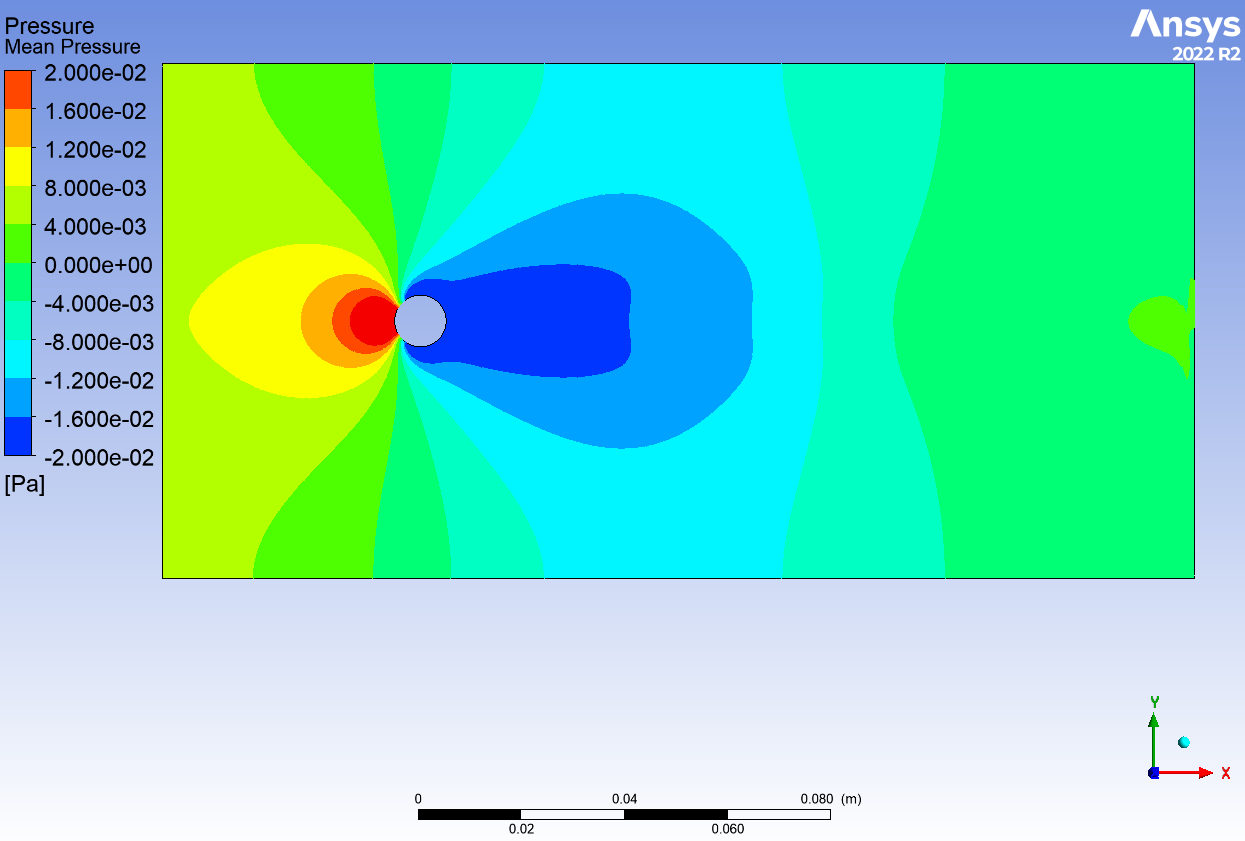
\includegraphics[width=0.8\textwidth]{Questions/Figures/mean pressure grid 3.png}
    \caption{Mean Pressure Contour for Grid 3}
\end{figure}

\subsubsection*{Grid 4}
\begin{figure}[H]
    \centering
    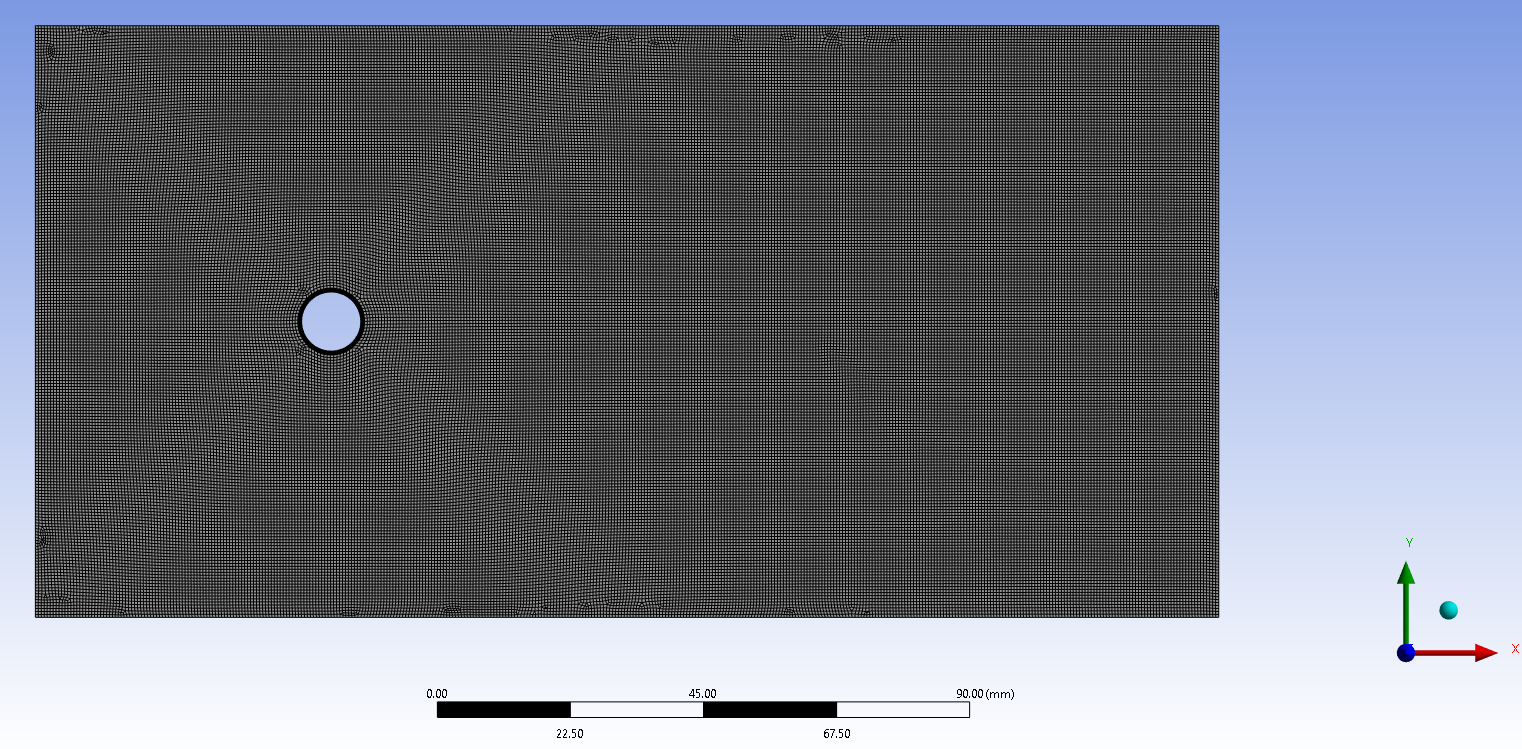
\includegraphics[width=0.8\textwidth]{Questions/Figures/mesh with grid 4.png}
    \caption{Mesh for Grid 4}
\end{figure}
\begin{figure}[H]
    \centering
    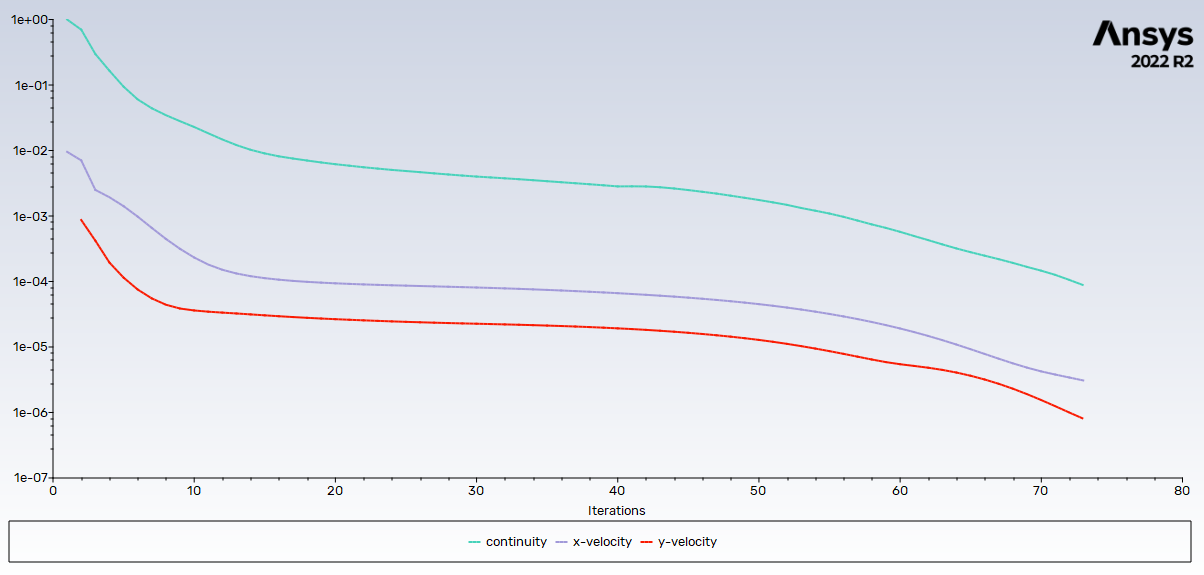
\includegraphics[width=0.8\textwidth]{Questions/Figures/residuals grid 4.png}
    \caption{Residuals for Grid 4}
\end{figure}
\begin{figure}[H]
    \centering
    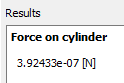
\includegraphics[width=0.8\textwidth]{Questions/Figures/force on cylinder grid 4.png}
    \caption{Mean Drag Force for Grid 4}
\end{figure}
By direct calculation, the mean drag coefficient is
\begin{align*}
    C_{d4} &= \frac{F_{D4}}{0.5\rho U_\infty^2 D} \\
    &= \frac{3.92433 \times 10^{-7}}{0.5 \times 1.184 \times 0.24^2 \times 0.1} \\
    &= 1.15 \times 10^{-4}
\end{align*}
From the plot, the recirculation length is approximately
\begin{align*}
    L_{r4} &= \frac{0.094 - 0.05}{0.001} \\
    &=\boxed{44.0}
\end{align*}
\begin{figure}[H]
    \centering
    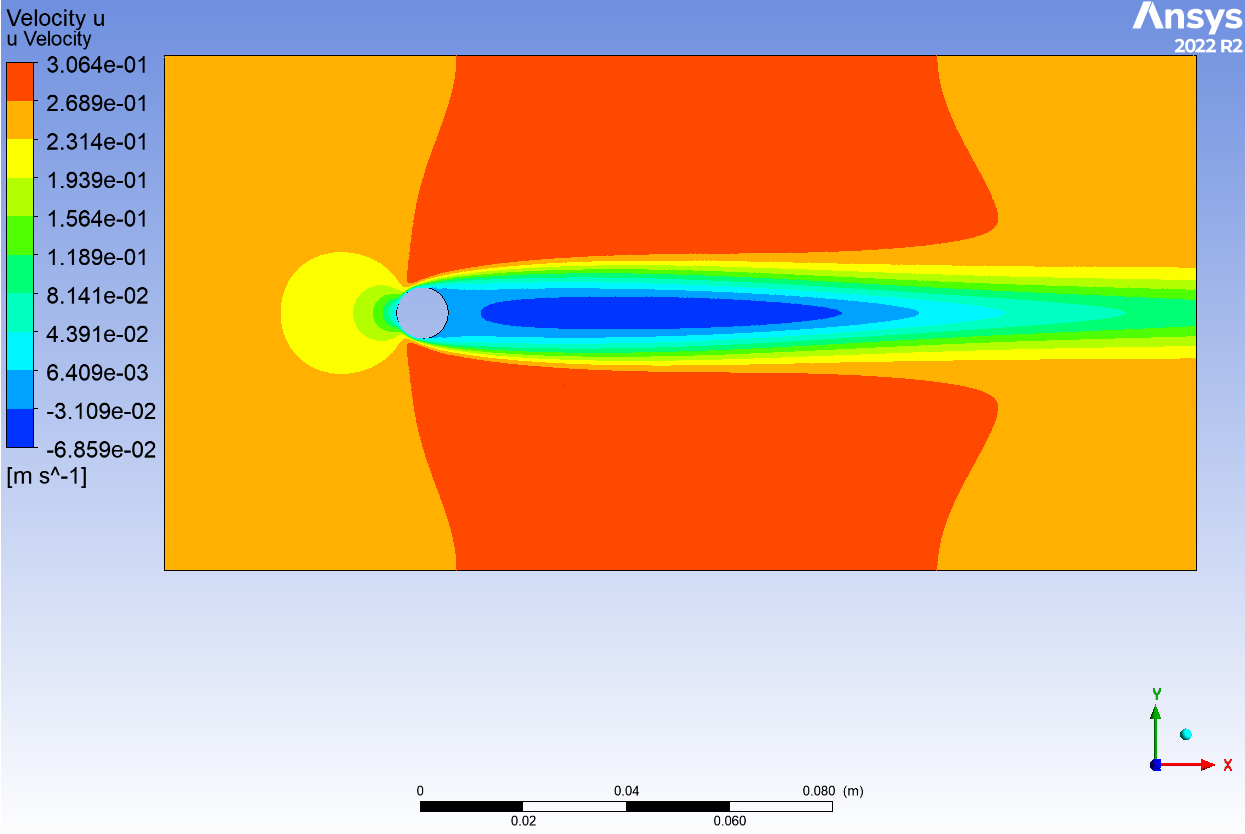
\includegraphics[width=0.8\textwidth]{Questions/Figures/u velocity contour grid 4.png}
    \caption{Mean Streamwise Velocity Contour for Grid 4}
\end{figure}
\begin{figure}[H]
    \centering
    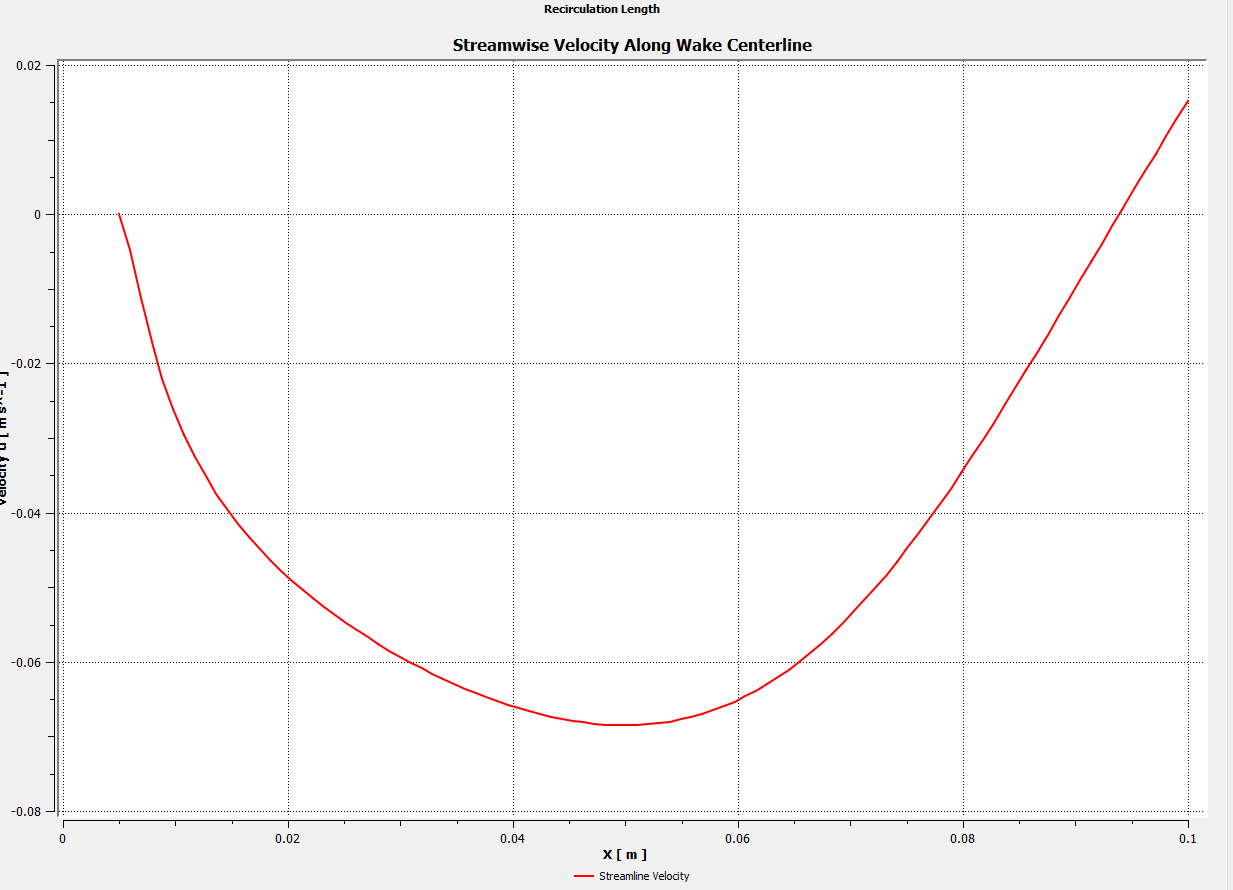
\includegraphics[width=0.8\textwidth]{Questions/Figures/plot with grid 4.png}
    \caption{Mean Streamwise Velocity for Grid 4}
\end{figure}
\begin{figure}[H]
    \centering
    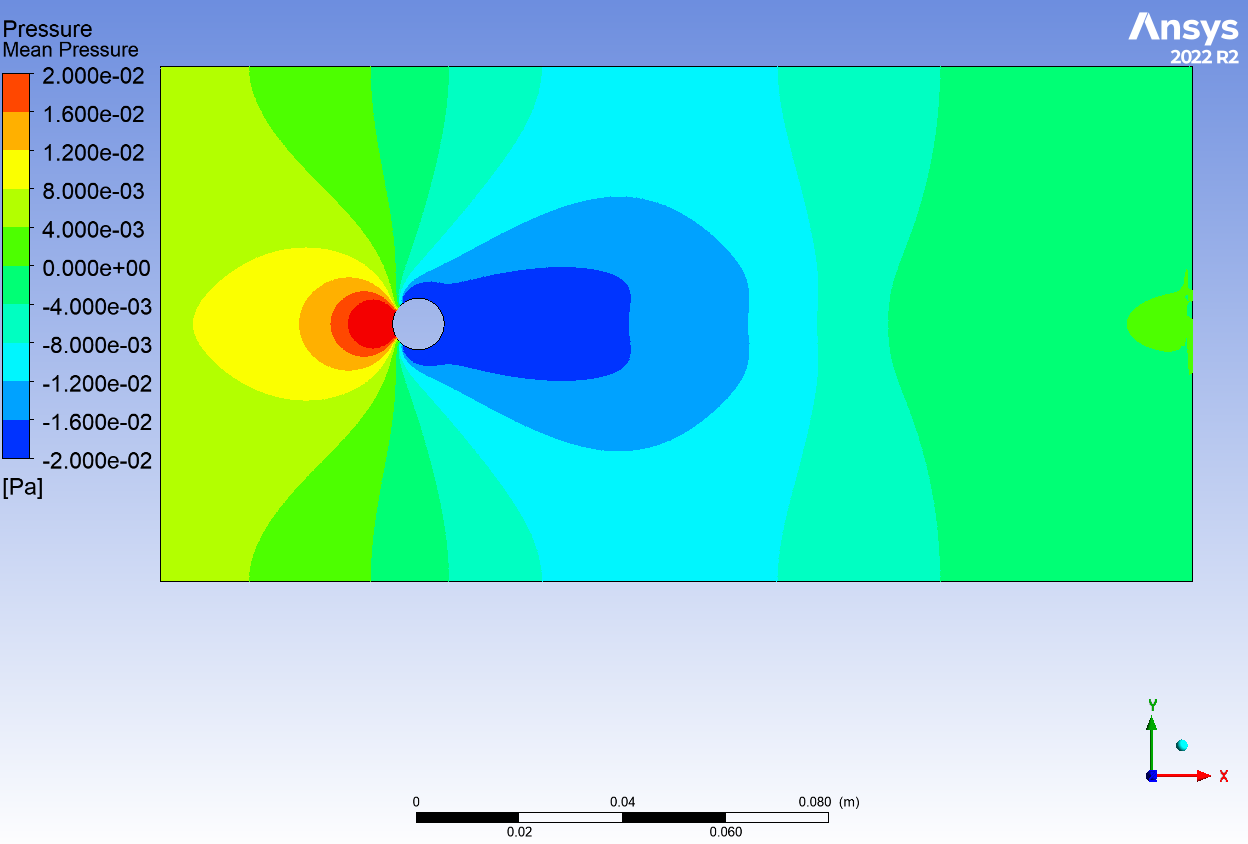
\includegraphics[width=0.8\textwidth]{Questions/Figures/mean pressure grid 4.png}
    \caption{Mean Pressure Contour for Grid 4}
\end{figure}